\subsection{Evaluating Cryptographic Building Blocks}\label{eva: microbenchmarks}

\begin{figure*}[t!]
    \begin{minipage}[t]{0.5\linewidth}
    \centering
    \begin{subfigure}[b]{0.5\textwidth}
    \centering
    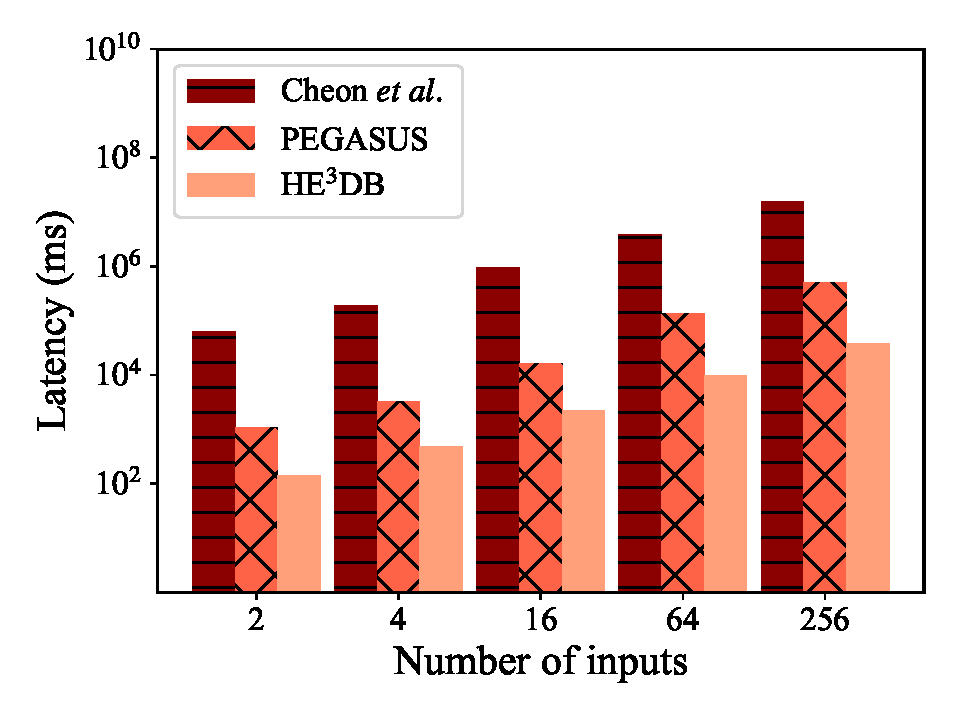
\includegraphics[width=\linewidth]{figure/minbench_4.pdf}
    % \vspace{-2em}
    \caption{4-bit $\dbmin$}
    \label{fig:homminbench4}
    \end{subfigure}%
    \hfill
    \begin{subfigure}[b]{0.5\textwidth}
    \centering
    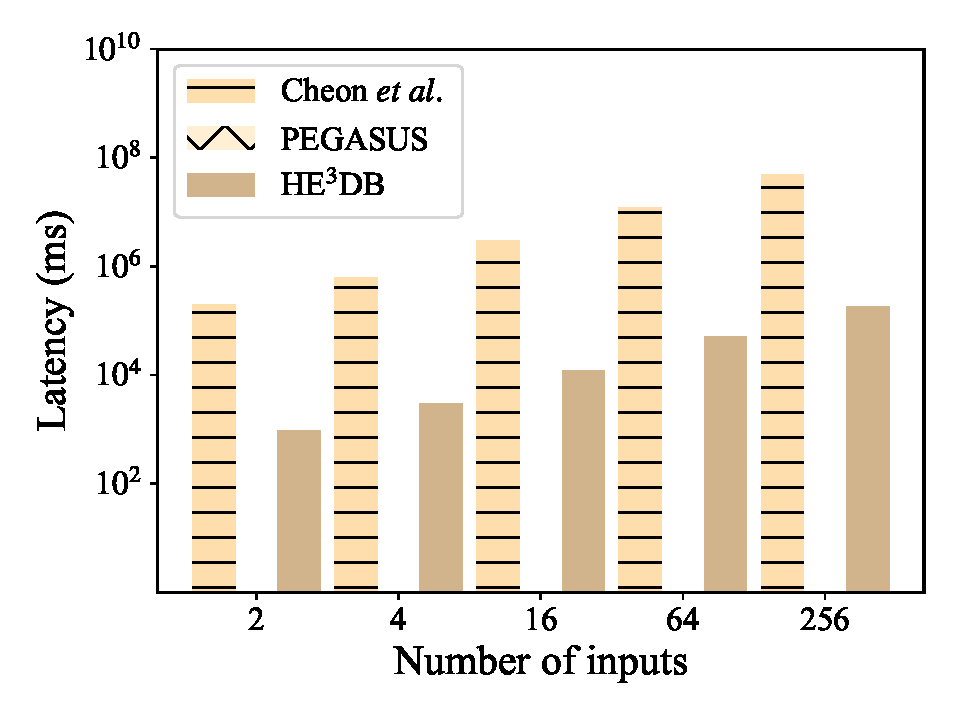
\includegraphics[width=\linewidth]{figure/minbench_16.pdf}
    % \vspace{-2em}
    \caption{16-bit $\dbmin$}
    \label{fig:homminbench16}
    \end{subfigure}%
    \caption{Benchmark results for Homomorphic $\dbmin$.}
    \Description{Benchmark results for Homomorphic $\dbmin$. The horizontal axis is the number of inputs, and the vertical axis is the latency. From the result, our performance is on average 
    around one order of magnitude faster than PEGASUS~\cite{pegasus}
    and two orders of magnitude faster than ~\cite{ckkscomparison}.}
    \label{fig: homminbench}
    \end{minipage}%
    \begin{minipage}[t]{0.5\linewidth}
    \centering
    \begin{subfigure}[b]{0.5\textwidth}
    \centering
    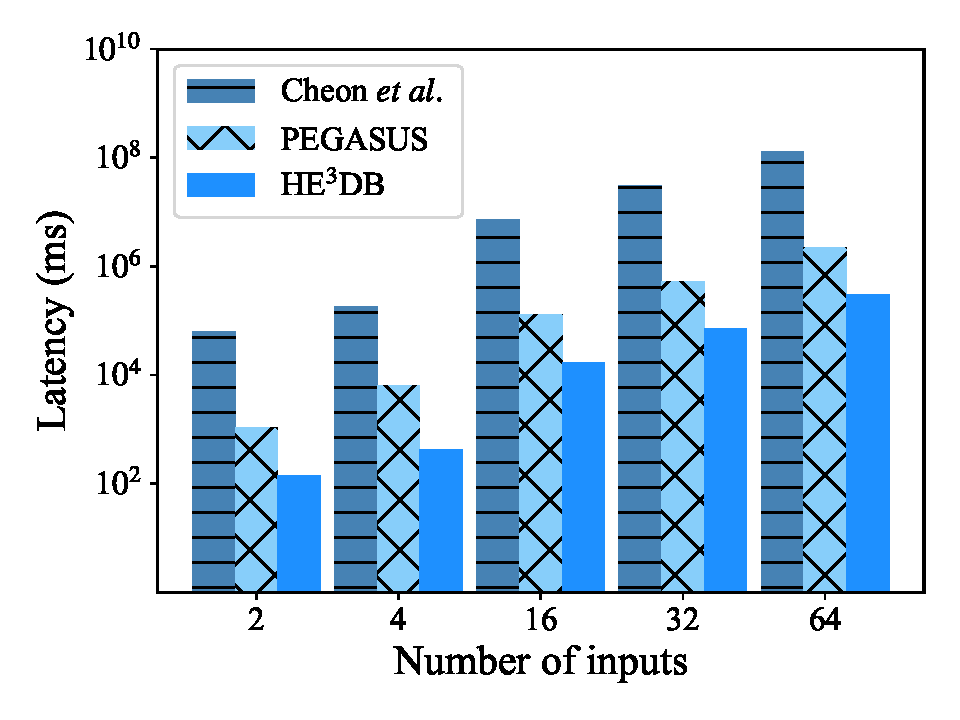
\includegraphics[width=\linewidth]{figure/sortbench_4.pdf}
    % \vspace{-2em}
    \caption{4-bit \orderby}
    \label{fig:homsortbench4}
    \end{subfigure}%
    \hfill
    \begin{subfigure}[b]{0.5\textwidth}
    \centering
    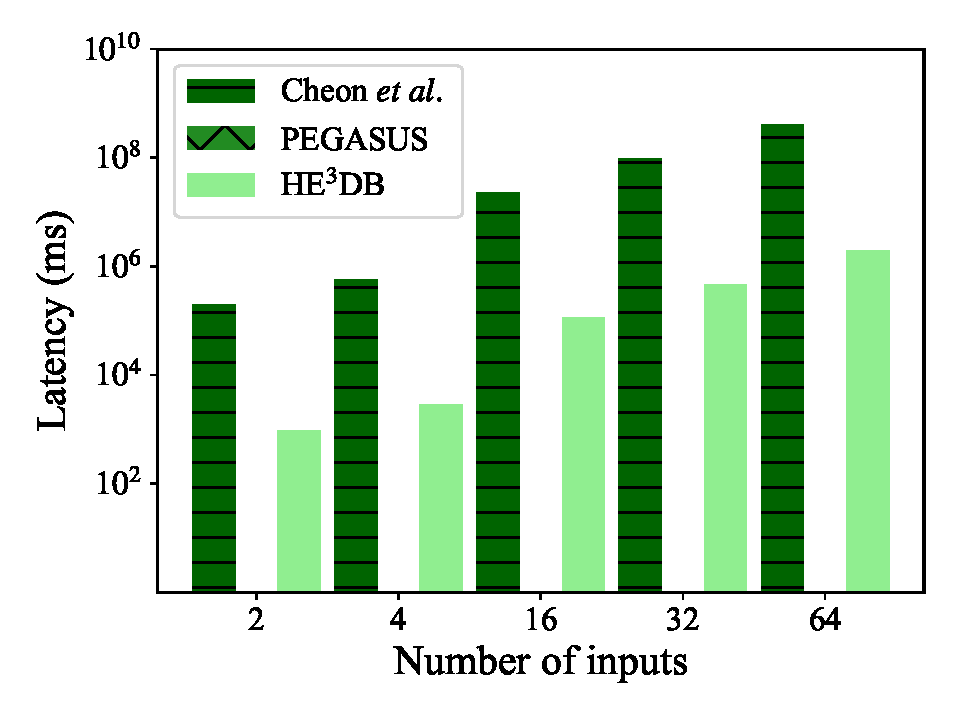
\includegraphics[width=\linewidth]{figure/sortbench_16.pdf}
    % \vspace{-2em}
    \caption{16-bit \orderby}
    \label{fig:homsortbench16}
    \end{subfigure}%
    \caption{Benchmark results for Homomorphic $\orderby$.}
    \Description{Benchmark results for Homomorphic $\orderby$. The horizontal axis is the number of inputs, and the vertical axis is the latency. From the results, our performance is on average 
    around one order of magnitude faster than PEGASUS~\cite{pegasus}
    and two orders of magnitude faster than ~\cite{ckkscomparison}.}
    \label{fig: homsortbench}
    \end{minipage}
   % \begin{center}
   %  \begin{subfigure}[b]{0.25\textwidth}
   %  \centering
   %  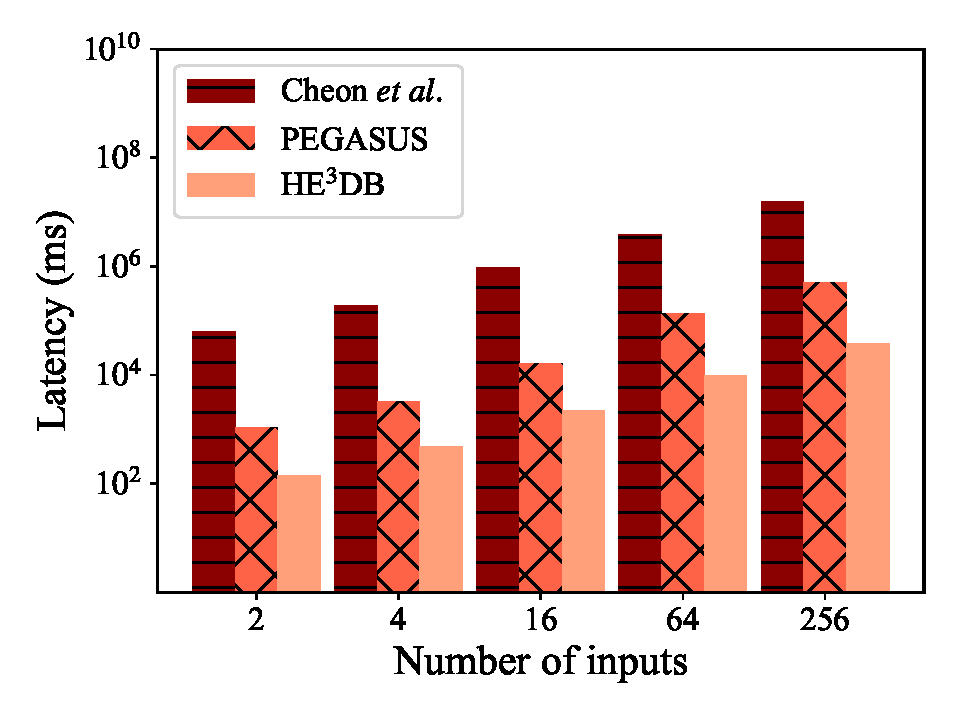
\includegraphics[width=\linewidth]{figure/minbench_4.pdf}
   %  % \vspace{-2em}
   %  \caption{4-bit}
   %  \label{fig:homminbench4}
   %  \end{subfigure}%
   %  \hfill
   %  \begin{subfigure}[b]{0.25\textwidth}
   %  \centering
   %  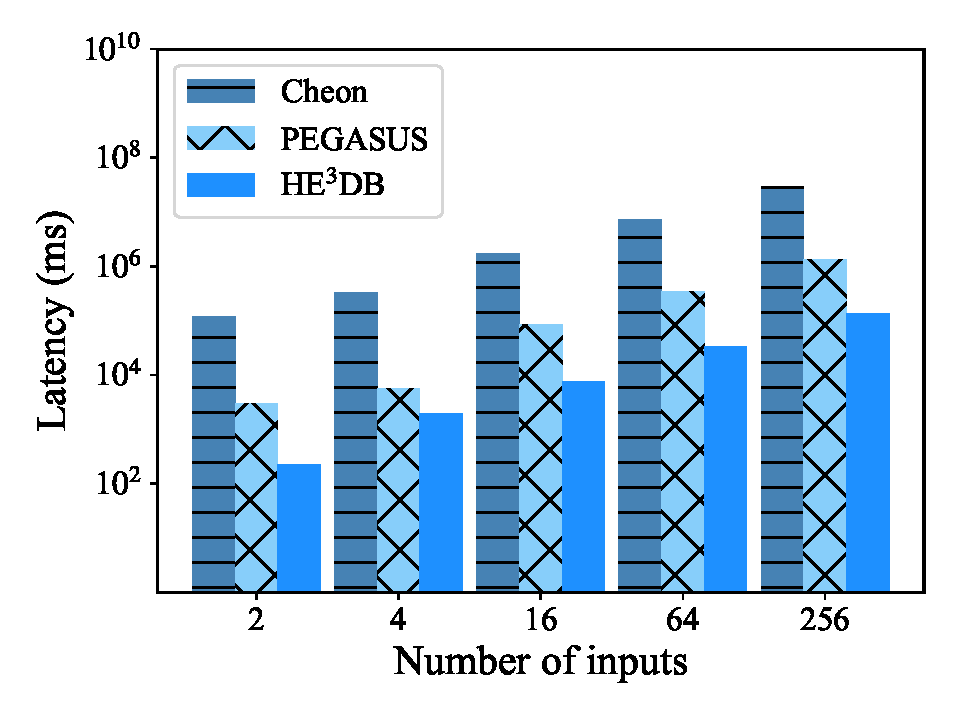
\includegraphics[width=\linewidth]{figure/minbench_8.pdf}
   %  % \vspace{-2em}
   %  \caption{8-bit}
   %  \label{fig:homminbench8}
   %  \end{subfigure}%
   %  \hfill
   %  \begin{subfigure}[b]{0.25\textwidth}
   %  \centering
   %  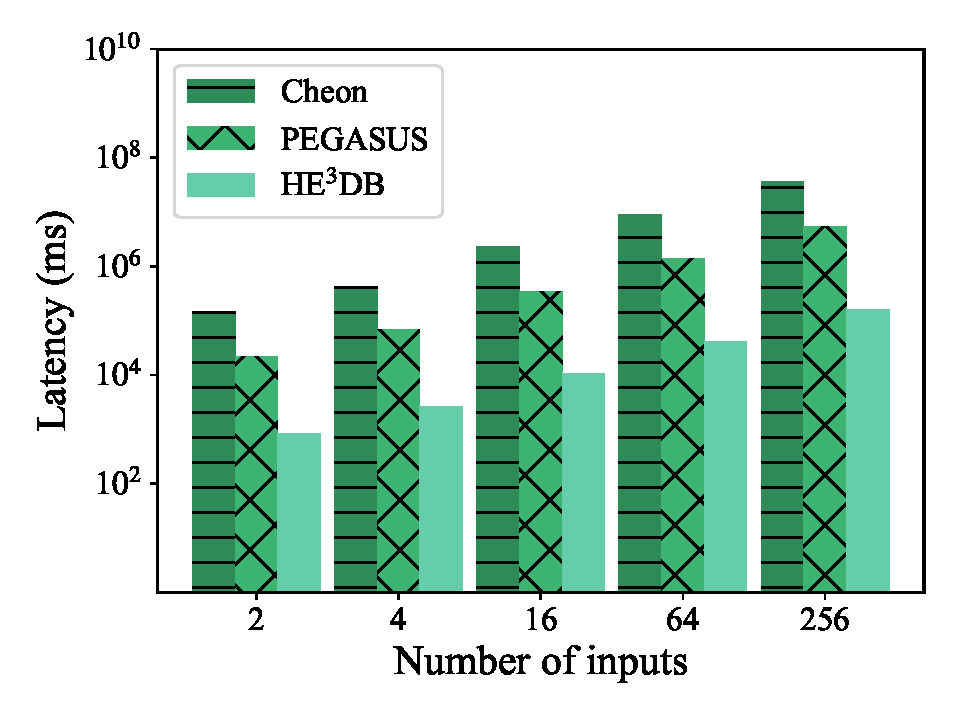
\includegraphics[width=\linewidth]{figure/minbench_12.pdf}
   %  % \vspace{-2em}
   %  \caption{12-bit}
   %  \label{fig:homminbench12}
   %  \end{subfigure}%
   %  \hfill
   %  \begin{subfigure}[b]{0.25\textwidth}
   %  \centering
   %  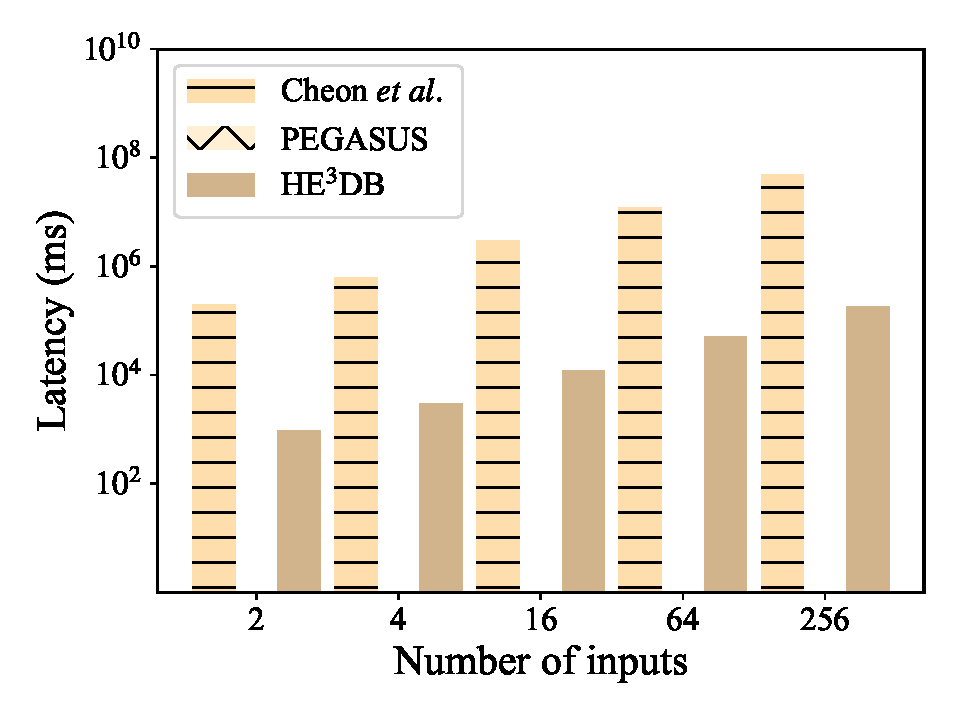
\includegraphics[width=\linewidth]{figure/minbench_16.pdf}
   %  % \vspace{-2em}
   %  \caption{16-bit}
   %  \label{fig:homminbench16}
   %  \end{subfigure}%
   
   % \end{center}
   %  % \vspace{-0.5em}
   %    \caption{Homomorphic MIN benchmark between $2,4,16,64,256$ numbers
   %          with $4,8,12$, and $16$ bits of precision.} 
   % \label{fig: homminbench}
   % \vspace{-0.5em}
\end{figure*}


%Here, we answer {\bf{RQ1}}. 
To answer {\bf{RQ1}}, we benchmark the efficiency of each of the 
cryptographic building blocks proposed in \cref{block},
including homomorphic comparison in \cref{block: comparison}, 
homomorphic \texttt{MIX/MAX} evaluation in \cref{block: minmax}
and ciphertext conversion in \cref{block: LWEsPack}. 
% The results
% are summarized as follows.

% {\bf{Homomorphic comparison}}:
%\subsubsection{Homomorphic comparison}
First of all, we compare the proposed $\homcomp$ with the best known 
existing works that support unbounded-depth predicate
evaluation, and the results are summarized in \cref{tab:combenchmark}.
We re-implement some of the existing works based on their open-source 
implementations~\cite{codepegasus, codesortinghat, codeopenfhe}
to fit our purpose (i.e., ciphertext-ciphertext comparison).
As observed in \cref{tab:combenchmark}, we are 7$\times$--113$\times$
faster than existing methods. Meanwhile, we can reduce the ciphertext
size by as much as 4.75$\times$ owing to our elastic ciphertext 
management policy.
% In addition,
% In \cref{tab:combenchmark}, we sketch the change
% of latency and ciphertext size on the predicate comparison operator $\geq$ 
% indifferent bits of precision.
% Specifically, in terms of latency, we achieve
% $24.67\times$, $19.07\times$, $8.13\times$ and $7.67\times$
% faster than the second best results on $4,8,12$, and $16$ bits of 
% precision, respectively.
In addition, as we can see from \cref{fig: homcompbench}, our
speedups are consistent across different comparison operators.
% shows the change of latency with 
% the increasing bits of precision for different methods. 
% As can be seen, our \NAME achieves lower latency
% compared to other methods on comparison operators $\geq, ==, >$, 
% which indicates higher efficiency.



%\subsubsection{Homomorphic \texttt{MIN/MAX}}
% {\bf{Homomorphic \dbmin/\dbmax}}: 
%\subsubsection{Homomorphic $\dbmin$/$\dbmax$ and $\orderby$}
Next, we compare the latency performance of the proposed homomorphic
\texttt{MIN/MAX} algorithms and SQL $\orderby$ operator to 
PEGASUS~\cite{pegasus} and Cheon \etal~\cite{ckkscomparison}
% and \NAME on the
% same numbers with the same bits of precision.
with a varying number of inputs and bit precision for the inputs.
As depicted in \cref{fig: homminbench} and \cref{fig: homsortbench},
our performance is on average around 
one order of magnitude faster than PEGASUS~\cite{pegasus},
and two orders of magnitude faster
than~\cite{ckkscomparison}.
Note in \cref{fig: homminbench} (b) and \cref{fig: homsortbench} (b) the 
histograms of PEGASUS~\cite{pegasus}
are left blank, for PEGASUS cannot support homomorphic \texttt{MIN/MAX} 
and $\orderby$ functions
over 16-bit operands.

%\subsubsection{Homomorphic ciphertext conversion}
% {\bf{Homomorphic Conversion}}: 
%\subsubsection{Homomorphic conversion}
% In ~\cref{tab:conversionbenchmark}, 
Lastly, to test the performance of the proposed $\repack$ operator, we
compare our algorithm to PEGASUS~\cite{pegasus} and 
Chen \etal~\cite{conversionhaochen}
over the task of converting $2^{15}$ LWE ciphertexts into
one RLWE ciphertext. Although PEGASUS~\cite{pegasus} achieves 
the lowest latency ($56s$), 
the method can only obtain $4$ bits of precision, which is 
not practical in most DB applications.
Although both the proposed $\repack$ and Chen \etal~\cite{conversionhaochen}
achieves higher precision ($\geq 16$ bits), \NAME
can be as much as $2 \times$ faster than~\cite{conversionhaochen}.

% \begin{table}[t!] 
%     \centering
%     \caption{Ciphertext converison benchmark}
%     \vspace{0em}
%         \begin{tabular}{ccc}
%             \toprule
%             Methods &  Precision (bit) & Latency (s)\\
%             \midrule
%             Pegasus~\cite{pegasus} &  4 & 56\\
%             Chen~\cite{conversionhaochen} & 20 & 230 \\
%             HE$^3$DB & 16 & 114 \\

%             \bottomrule
%         \end{tabular}
%     \label{tab:conversionbenchmark}
% \end{table}

